%
% dtf.tex -- Idee mit DFT
%
\section{Übertragung mit Hilfe der Diskrten Fourier-Transformation
\label{reedsolomon:section:dtf}}
\rhead{Umwandlung mit DTF}
Die Grundidee eines fehlerkorrigierenden Code ist, dass Informationen eines Datenpunkt, 
durch die Codierung, auf viele übertragene Werte verteilt werden.
Die Decodierung ist in der Lage, den ursprünglichen Datenwert zu rekonstruieren,
sogar wenn einzelne wenige übertragene Werte beschädigt worden sind.
\par
Die Fourier-Transformation transformiert einen einzelnen Wert, 
eine Dirac-Funktion, auf ein Spektrum, welches sich über die ganze Frequenzachse erstreckt.
Aus der Filtertheorie ist bekannt, dass der ursprüngliche Impuls mehr oder weniger rekonstruierbar ist.
Forausgestzt, es gehen nicht zu viele Frequenzen bei der Übertragung verloren.
\par
Es liegt daher nahe zu versuchen, die Fourier-Transformation 
für Codierung und Decodierung zu verwenden.

\subsection{Beispiel mit Fehlerkorrektur mit Fourier-Transformation
\label{reedsolomon:subsection:sendbsp}}

Das folgende Beispiel soll zeigen, wie Fehlerkorrektur möglich ist.
Dieses auf eine Art, die der Funktionsweise des Reed-Solomon-Codes,
der später erklärt wird, analog ist.
\par
Der Auftrag ist nun 64 Daten zu übertragen, 32 Fehler erkennen und 16 Fehler rekonstruieren.
Mit hilfe der Fourier-Transformation werden die \textcolor{blue}{blauen Datenpunkte} transformiert,
zu den \textcolor{darkgreen}{grünen Übertragungspunkten}. 
Durch eine Rücktransformation könnnen die \textcolor{blue}{blauen Datenpunkte} wieder rekonstruiert werden.

\begin{figure}
	\centering
	\resizebox{\textwidth}{!}{
	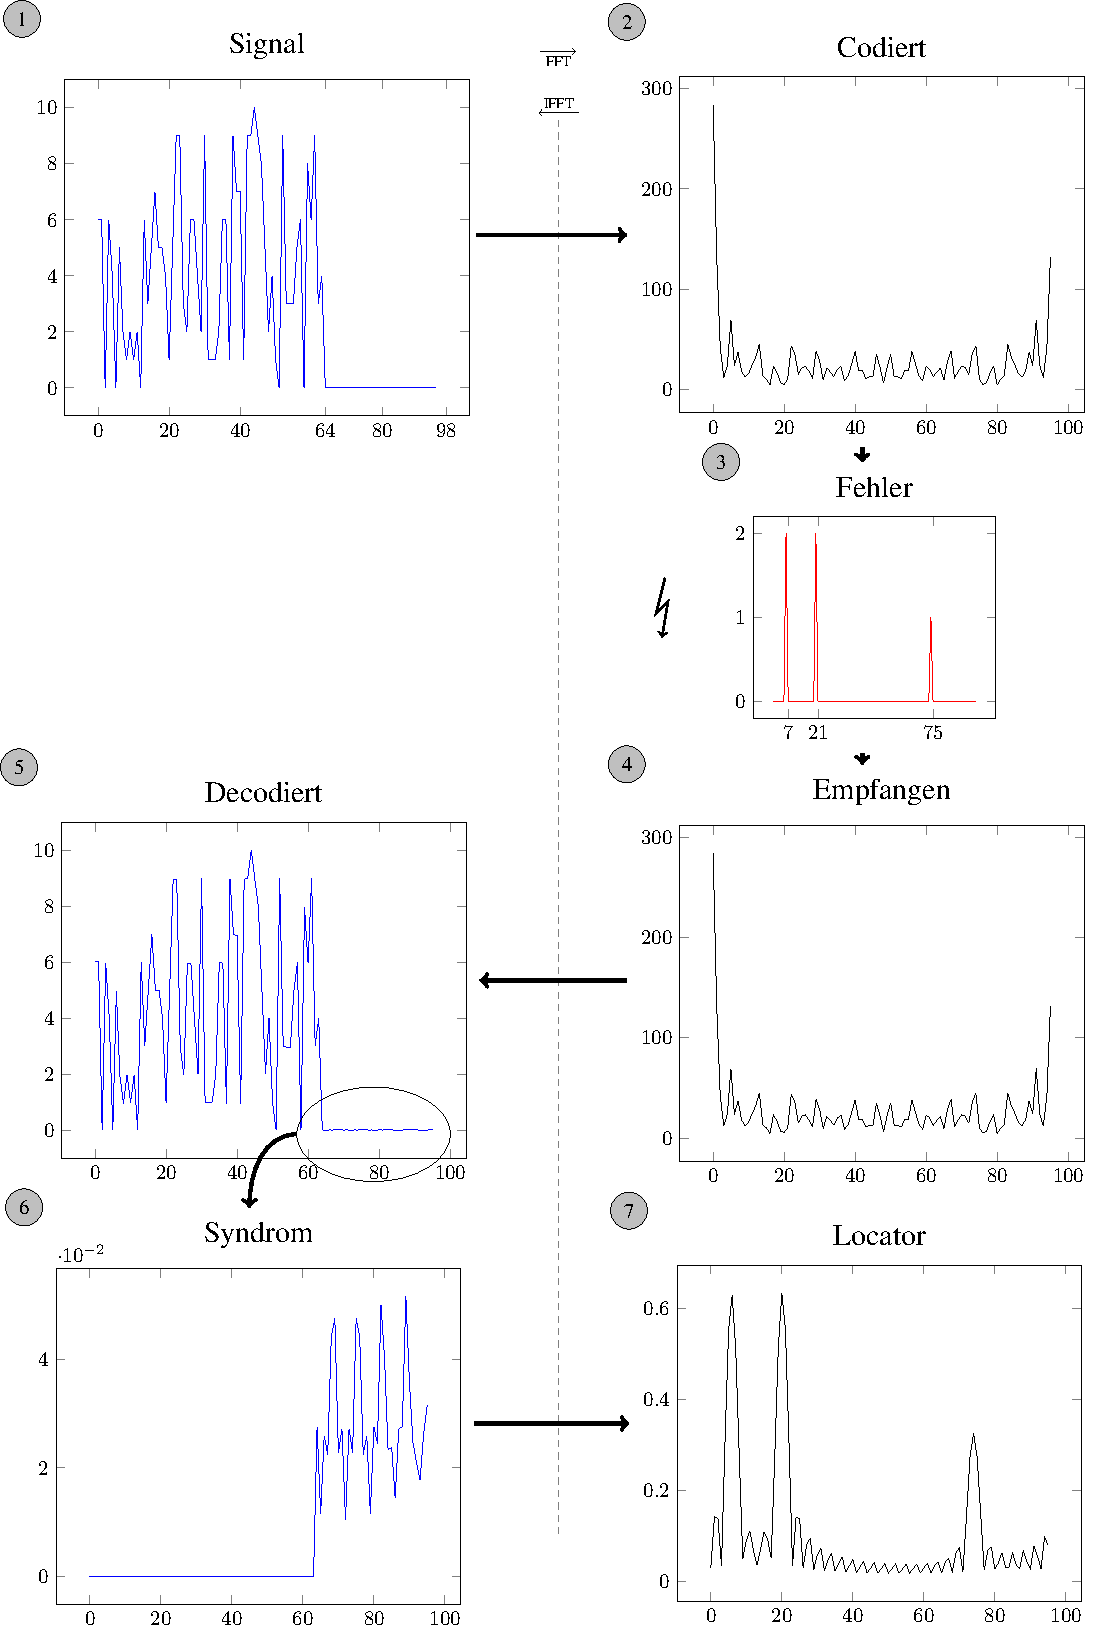
\includegraphics[width=\textwidth]{papers/reedsolomon/figures/plotfft}
    %
\begin{tikzpicture}[]

	%---------------------------------------------------------------
	%Knote
	\matrix(m) [draw = none, column sep=25mm, row sep=2mm]{

		\node(signal)  []    {
		\begin{tikzpicture}
			\begin{axis}
				[title = {\Large {Signal}}, 
				xtick={0,20,40,64,80,98}]
				\addplot[blue] table[col sep=comma] {tikz/signal.txt};
			\end{axis}
		\end{tikzpicture}}; &
		
		\node(codiert) []    {
		\begin{tikzpicture}[]
			\begin{axis}[ title = {\Large {Codiert \space + \space Fehler}},
				xtick={0,40,60,100}, axis y line*=left]
				\addplot[green] table[col sep=comma] {tikz/codiert.txt};
			\end{axis}
			\begin{axis}[xtick={7,21,75}, axis y line*=right]
					\addplot[red] table[col sep=comma] {tikz/fehler.txt};
			\end{axis}
		\end{tikzpicture}}; \\
		
		\node(decodiert) []    {
		\begin{tikzpicture}
			\begin{axis}[title = {\Large {Decodiert}}]
				\addplot[blue] table[col sep=comma] {tikz/decodiert.txt};
			\end{axis}
		\end{tikzpicture}}; &
	
		\node(empfangen) []    {
		\begin{tikzpicture}
			\begin{axis}[title = {\Large {Empfangen}}]
				\addplot[green] table[col sep=comma] {tikz/empfangen.txt};
			\end{axis}
		\end{tikzpicture}};\\
	
		\node(syndrom) []   {
		\begin{tikzpicture}
			\begin{axis}[title = {\Large {Syndrom}}]
				\addplot[black] table[col sep=comma] {tikz/syndrom.txt};
			\end{axis}
		\end{tikzpicture}}; &
	
		\node(locator) []    {
		\begin{tikzpicture}
			\begin{axis}[title = {\Large {Locator}}]
				\addplot[gray] table[col sep=comma] {tikz/locator.txt};
			\end{axis}
		\end{tikzpicture}};\\
	};
	%-------------------------------------------------------------
		%FFT & IFFT deskription
	
	\draw[thin,gray,dashed] (0,9) to (0,-9);
	\node(IFFT)  [scale=0.9]  at (0,9.3)   {IFFT};
	\draw[stealth-](IFFT.south west)--(IFFT.south east);
	\node(FFT)  [scale=0.9, above of=IFFT]    {FFT};
	\draw[-stealth](FFT.north west)--(FFT.north east);
	
	\draw[thick, ->,] (codiert)++(-1,0) +(0.05,0.5) -- +(-0.1,-0.1) -- +(0.1,0.1) -- +(0,-0.5);
	%Arrows
	\draw[thick, ->] (signal.east) to (codiert.west);
	\draw[thick, ->] (codiert.south) to (empfangen.north);
	\draw[thick, ->] (empfangen.west) to (decodiert.east);
	\draw[thick, ->] (syndrom.east) to (locator.west);
	\draw[thick](decodiert.south east)++(-1.8,1)  ellipse (1.3cm and 0.8cm) ++(-1.3,0) coordinate(zoom) ;
	\draw[thick, ->] (zoom) to[out=180, in=90] (syndrom.north);
	
	%item
	\node[circle, draw, fill =lightgray] at (signal.north west) {1};
	\node[circle, draw, fill =lightgray] at (codiert.north west) {2+3};
	\node[circle, draw, fill =lightgray] at (empfangen.north west) {4};
	\node[circle, draw, fill =lightgray] at (decodiert.north west) {5};
	\node[circle, draw, fill =lightgray] at (syndrom.north west) {6};
	\node[circle, draw, fill =lightgray] at (locator.north west) {7};
\end{tikzpicture}	
	}
	\caption{Übertragungsabfolge \ref{reedsolomon:subsection:sendbsp}}
	\label{fig:sendorder}
\end{figure}
In der Abbildung \ref{fig:sendorder} wird eine Übertragung Schritt für Schritt illustriert.
In der folgenden Aufzählung werden diese einzelne Schritte erklärt und erläutert:
\begin{enumerate}[(1)]
 \item Das Signal ist mit 64 zufälligrn, ganzzahligen Datenwerten, zwischen 0 und 10.
 Für die Rekonstruktion werden zusäzlich Datenwert benötigt, wir fügen deshalb 32 Werte hinzu.
 Diese setzen wir willkürlich auf Null und nennen sie Fehlerkorrekturstellen
 \externaldocument{papers/reedsolomon/idee}\ref{reedsolomon:section:Fehlerkorrekturstellen}.
 Wir erhalten so einen erweiterten Signalvektor der länge $N =96$.
 \item Mit der Fourier-Transformation wird der ganze Signalvektor codiert.
 Dadurch wird jede Informationseinheit auf alle Punkte des Spektrums verteilt.
 \item Wir dürfen annehmen, dass bei der Übertragung, nur einzelne übertragene Werte durch Fehler,
 verändert werden.
 \par 
 Im Beispiel sind dies die Werte an den Stellen 7, 21 und 75(\textcolor{red}{rote Kurve}),
 die um einen Betrag verändert werden.
 Dieser ist bis zu 150-mal kleiner, als die ursprünglichen codierte Werte. 
 Der Empfänger kennt daher im allgemeinen nicht, ob und wo Übertragungsfehler aufgetreten sind.
 \item Ohne Übertragungsfehler kann der Signalvektor durch Inverse Fourier-Transformation vollständig
 wiederhergestellt werden.
 Dazu gehören auch die Nullen an den Fehlerkorrekturstellen 64 - 96.
 \par 
 Sind Übertragungsfehler aufgetreten, werden an diesen Stellen, Werte abweichend von Null, auftreten.
 Somit haben wir bereits Fehler erkannt.
 \item Die Werte an den Fehlerkorrekturstellen 64 - 96, die nicht mehr Null sind, nennenwir das Syndrom.
 Im Syndrom steckt nur Information über die Fehler, sie werden durch die Inverse Fourier-Transformation erzeugt.
 \item Um die Fehler zu rekonstruieren, ann man versuchen, die Information im Syndrom mit Fourier-Transformation zu transformieren.
 Da das Syndrom nur ein Teil der Fehlerinformation ist, liefert die Fourier-Transformation eine Approximation der Fehler.
 Diese Approximation der Fehler ist genau genug, um die Fehlerstellen zu localisieren.
\end{enumerate}
Im Beispiel haben wir mit dem Syndrom nur etwa ein Drittel der Fehlerinformation, es ist daher zu erwarten, 
dass die Fehlerwerte auch nur ein drittel so gross sind.
\par 
Damit können die Fehler korrigiert und die Orginaldaten wiederhergestellt werden.
Der Rekonstruktionsauftrag ist damit erfolgreich ausgeführt.

\subsection{Fourier-Transformation und Polynome\label{reedsolomon:subsection:ftandpolynom}}
Im Abschnitt \externaldocument{papers/reedsolomon/idee}\ref{reedsolomon:section:polynomansatz}
wurden Werte eines Polynoms zur Codierung verwendet.
Die 7 Übertragungspunkte könnten ein Polynom
\begin{equation}
	\textcolor{darkgreen}{p(x)}
	=
	\textcolor{blue}{a_0} + \textcolor{blue}{a_1}x + \textcolor{blue}{a_2}x^2 +
	\textcolor{gray}{a_3}x^3 + \textcolor{gray}{a_4}x^4 + \textcolor{gray}{a_5}x^5 +
	\textcolor{gray}{a_6}x^6
\label{reedsolomon:equationpoly}
\end{equation}
sechsten Grades bestimmen.
Durch die Wahl von $\textcolor{gray}{a_3=0}$, $\textcolor{gray}{a_4=0}$, $\textcolor{gray}{a_5=0}$, $\textcolor{gray}{a_6=0}$ 
erzeugen wir die, für die Fehlerkorrektur,
nötige Redundanz, ganz analog zum Schritt (1) im Beispiel.
\par 
Die Analogie geht aber noch weiter.
 Schreibt man 
 \( w =
 e^{-\frac{2\pi j}{N} k}\)
 \label{reedsolomon:DFT_summand}, damit wird aus der Formel
 \begin{equation}
	\hat{c}_{k} 
	= \frac{1}{N} \sum_{n=0}^{N-1}
	{f}_n \cdot e^{-\frac{2\pi j}{N} \cdot kn}
	,\label{reedsolomon:DFT}
 \end{equation}
 für die Diskrte-Fourier-Transformation das Polynom
 \begin{equation}
	q(w)=
	\frac{{f}_0}{N} + \frac{{f}_1}{N} w^1 + \frac{{f}_2}{N} w^2 + \dots + \frac{{f}_{N-1}}{N} w^{N-1}
	\label{reedsolomon:DFT_polynom}
 \end{equation}
 Im Beispiel werden aber Werte des des Polynoms $q(w)$ für verschieden 
 \( w = e^{-\frac{2\pi j}{N} k}, k=1, \dots , k=N-1\) übermittelt.
 \begin{equation}
	\textcolor{darkgreen}{q(w)}=
	\frac{\textcolor{blue}{{f}_0}}{N} + \frac{\textcolor{blue}{{f}_1}}{N} w^1 + \frac{\textcolor{blue}{{f}_2}}{N} w^2 + \dots + 
	\frac{\textcolor{blue}{{f}_{63}}}{N} w^{63} + \frac{\textcolor{gray}{{f}_{64}}}{N} w^{64} + \textcolor{gray}{\dots} + \frac{\textcolor{gray}{{f}_{N-1}}}{N} w^{N-1}
	\label{reedsolomon:DFT_polynom2}
 \end{equation}
Das syndrom entstand durch die Wahl ${f_{64}}=0$ bis ${f}_{N-1}=0$.(graue koeffizenten)
\par
Die Polynominterpolation und die Fourier-Transformation rechnen beide mit reelen Zahlen.
Wenn die Approximation nicht mehr genügend gut ist um die Fehler zu erkennen und rekonstruieren,
dann müssen wir von den Reelen-Zahlen weg und zum endlichen Körpern, oder auch Galios-Körper genannt.
Deshalb haben die Mathematiker einen neuen Körper gesucht und ihn in der Endlichkeit gefunden,
dies wird nun im nächsten Abschnitt genauer erklärt.

